% MycoFlow Validation Technical Report — supplementary to the IEEE TCE submission
% Compiles independently. Embeds all three test-run artefacts.
% Build: pdflatex validation_report.tex (twice for refs)

\documentclass[11pt,a4paper]{article}

\usepackage[margin=2.2cm]{geometry}
\usepackage{amsmath,amssymb}
\usepackage{graphicx}
\usepackage{booktabs}
\usepackage{multirow}
\usepackage{array}
\usepackage[table]{xcolor}
\usepackage{hyperref}
\usepackage{caption}
\usepackage{titlesec}
\usepackage{enumitem}
\usepackage{tabularx}

\hypersetup{
  colorlinks,
  linkcolor=blue!50!black,
  urlcolor=blue!50!black,
  citecolor=red!40!black,
}

\titleformat{\section}{\Large\bfseries\color{blue!40!black}}{\thesection}{0.6em}{}
\titleformat{\subsection}{\large\bfseries}{\thesubsection}{0.6em}{}

\setlist{noitemsep, topsep=4pt}

\title{\textbf{MycoFlow: In-Vivo Validation Technical Report}\\
       \large Supplementary material to the IEEE TCE submission}
\author{Bar\i{}\c{s} Can Atakl\i{}\\\small\texttt{bariscanatakli@gmail.com}}
\date{April 2026}

\begin{document}
\maketitle

\begin{abstract}
\noindent
This technical report supplements the IEEE Transactions on Consumer
Electronics submission \emph{``MycoFlow: A Bio-Inspired Reflexive QoS
System for Consumer Routers with In-Vivo DNS-Aware Classification''}.
It provides the full per-class precision/recall tables, confusion
matrices, and hardware-resource timelines for three independently
executed in-vivo blind-replay runs (one WSL2 testbed, two Ubuntu
bare-metal runs differing only in the deployed DNS catalog), plus the
offline temporal-split validation that rules out heuristic overfitting.
All artefacts are reproducible from the project repository at
\href{https://github.com/bariscanatakli/mycoflow-core}{github.com/bariscanatakli/mycoflow-core}
under the same random seed (\texttt{seed=42}).
\end{abstract}

\section{Test Methodology}

\subsection{Stratified Random Per-Flow Replay}

\begin{itemize}
\item \textbf{Source dataset:} Universidad del Cauca April--June 2019
Network Flows (2{,}704{,}839 raw rows, 2{,}439{,}798 with a known
ground-truth label).
\item \textbf{Sampling:} stratified random, $N=150$ flows per service
class, 11 classes $\rightarrow$ 1{,}650 flows per run.
\texttt{numpy.random.seed(42)} for reproducibility.
\item \textbf{Replay primitives:} preserve per-flow $(\text{proto},
\text{dport}, \overline{\text{pkt\_size}}, \overline{\text{bw\_bps}})$
exactly. Bandwidth capped at 10\,Mbps to respect the testbed's uplink.
\item \textbf{Per-flow attribution:} 5-tuple \texttt{(src, dst, sport,
dport, proto)} match against the daemon's \texttt{state.flows[]} dump
$\Rightarrow$ each test flow is isolated from concurrent host traffic.
\end{itemize}

\subsection{Two Operating Modes}

\begin{description}
\item[\textbf{Mode A (control)}:] traffic emitted directly to a fixed
reachable target (\texttt{8.8.8.8} for UDP, \texttt{1.1.1.1} for TCP).
No DNS query for the persona-specific hostname is issued; the daemon's
DNS cache contains no entry that could hint $h_{dns}$. Verdict reduces
to $\arg\max(w_{port}, w_{beh})$.

\item[\textbf{Mode B (treatment)}:] before each flow, the laptop issues
a DNS A-record query for a representative service hostname to a public
resolver (\texttt{1.1.1.1}). The query and response transit the router;
the daemon's \texttt{AF\_PACKET} sniffer captures the response,
populates the IP$\rightarrow$service cache, and the test traffic then
goes to the resolved IP. Verdict has access to $h_{dns}$.
\end{description}

\subsection{Three Reported Metrics}

We report three accuracy levels because they answer different questions:

\begin{description}
\item[\textbf{Service-level (11-class):}] strict label match against
the Unicauca ground truth. The harshest metric: a video flow tagged
\texttt{video\_live} but classified as \texttt{video\_vod} counts as
wrong, even though the router places both in the same CAKE Video tin.

\item[\textbf{Tin-level (4-class):}] match collapses sibling labels by
their CAKE diffserv4 tin assignment (Voice / Video / Best-effort / Bulk).
This is what the router \emph{actually does} for the user; service-level
disagreements within one tin do not affect the user-visible outcome.

\item[\textbf{Tin-matched:}] tin-level accuracy restricted to flows the
classifier successfully observed (\texttt{flow\_matched=True}). This
is the ``deployment-realistic'' operating point: when the daemon sees
a flow at all, this is the fraction it places in the correct tin.
\end{description}

\section{Run Inventory}

\begin{table}[h]
\centering
\caption{Five in-vivo runs, all $N=1650$ stratified random sample with
\texttt{seed=42}.}
\begin{tabularx}{\textwidth}{lXcc}
\toprule
\textbf{Run ID} & \textbf{Description} & \textbf{Catalog} & \textbf{Date} \\
\midrule
WSL Mode A     & WSL2 client, NAT'd Ethernet, no DNS prime           & 80    & 2026-04-25 \\
WSL Mode B     & WSL2 client, organic DNS via 1.1.1.1                & 80    & 2026-04-25 \\
Ubuntu Mode A  & 1\,Gbps direct LAN, no DNS prime                    & 80    & 2026-04-26 \\
Ubuntu Mode B  & Direct LAN, organic DNS                             & 80    & 2026-04-27 \\
\textbf{Ubuntu Mode B (v2)} & \textbf{Same Ubuntu host, expanded catalog}    & \textbf{585}   & \textbf{2026-04-27} \\
\bottomrule
\end{tabularx}
\end{table}

\section{Headline Results}

\begin{table}[h]
\centering
\caption{Overall accuracy with Wilson 95\% CI, all five runs.}
\label{tab:overall}
\begin{tabular}{l|ccc}
\toprule
\textbf{Run} & \textbf{Service-acc} & \textbf{Tin-acc} & \textbf{Tin-matched} \\
\midrule
WSL    Mode~A           & 20.00\% [18.1,22.0] & 30.42\% [28.3,32.7] & 49.46\% [45.9,53.1] \\
WSL    Mode~B           & 32.48\% [30.3,34.8] & 45.39\% [43.0,47.8] & 64.42\% [61.3,67.4] \\
Ubuntu Mode~A           & 20.24\% [18.4,22.3] & 30.61\% [28.4,32.9] & 49.26\% [45.7,52.8] \\
Ubuntu Mode~B (80-cat.) & 33.39\% [31.2,35.7] & 48.61\% [46.2,51.0] & 66.97\% [64.0,69.8] \\
\rowcolor{blue!8} \textbf{Ubuntu Mode~B (585-cat.)} & \textbf{37.88\%} [35.6,40.3] & \textbf{52.42\%} [50.0,54.8] & \textbf{70.41\%} [67.6,73.1] \\
\bottomrule
\end{tabular}
\end{table}

\subsection{Three Independent Confirmations of the DNS Lift}

\begin{enumerate}
\item \textbf{Testbed invariance.} Mode~A is platform-invariant: WSL2
vs Ubuntu agree to within $|\Delta| < 0.5$\,pt across all three
metrics. The DNS lift is therefore not a network-stack artefact.

\item \textbf{Both testbeds show the lift.} WSL: $+12.5$\,pt service,
$+15.0$\,pt tin-matched. Ubuntu (80-cat.): $+13.2$\,pt and $+17.7$\,pt.
Ubuntu (585-cat.): $+17.6$\,pt and $+21.2$\,pt.

\item \textbf{Catalog scaling.} Going from 80 to 585 catalog entries
on the same Ubuntu host preserves the lift direction and increases
its magnitude — the gain is monotone in catalog coverage.
\end{enumerate}

\subsection{McNemar Pairing Tests}

\begin{table}[h]
\centering
\caption{Paired McNemar test (continuity-corrected $\chi^2$, df=1).
$b$ = Mode~B correct, Mode~A wrong; $c$ = Mode~A correct, Mode~B wrong.
$c=0$ in every run: DNS never \emph{degrades} the verdict.}
\begin{tabular}{l|cccc}
\toprule
\textbf{Run} & $\boldsymbol{\chi^2}$ & $\boldsymbol{p}$ & $\boldsymbol{b}$ & $\boldsymbol{c}$ \\
\midrule
WSL                & 204.00 & $5.0\!\times\!10^{-45}$ & 206 & 0 \\
Ubuntu (80-cat.)   & 215.00 & $2.1\!\times\!10^{-47}$ & 217 & 0 \\
\rowcolor{blue!8} Ubuntu (585-cat.) & \textbf{289.00} & $\boldsymbol{1.8\!\times\!10^{-63}}$ & \textbf{291} & \textbf{0} \\
\bottomrule
\end{tabular}
\end{table}

\section{Per-Class Breakdown — Final Run}

\begin{table}[h]
\centering
\caption{Per-class precision/recall, Ubuntu testbed, 585-catalog,
seed 42. $\Delta$ Rec. is the lift over the same testbed's Mode~A.}
\label{tab:perclass-final}
\begin{tabular}{l|cc|cc|c}
\toprule
\textbf{Class} & \multicolumn{2}{c|}{\textbf{Mode A}} & \multicolumn{2}{c|}{\textbf{Mode B}} & $\Delta$ \\
 & Prec. & Rec. & Prec. & Rec. & Rec. \\
\midrule
voip\_call        & 0.286 & 0.013 & 1.000 & 0.013 & +0.000 \\
game\_rt          & 0.829 & 0.227 & 0.567 & \textbf{0.760} & \textbf{+0.533} \\
video\_conf       & 1.000 & 0.893 & 0.716 & \textbf{0.993} & +0.100 \\
video\_live       & 1.000 & 0.007 & 1.000 & 0.020 & +0.013 \\
video\_vod        & 0.000 & 0.000 & 0.652 & \textbf{0.860} & \textbf{+0.860} \\
bulk\_dl          & 0.000 & 0.000 & 0.000 & 0.000 & +0.000 \\
file\_sync        & 0.000 & 0.000 & 1.000 & \textbf{0.433} & \textbf{+0.433} \\
torrent           & 1.000 & 0.227 & 1.000 & 0.227 & +0.000 \\
game\_launcher    & 0.000 & 0.000 & 0.000 & 0.000 & +0.000 \\
web\_interactive  & 0.000 & 0.000 & 0.000 & 0.000 & +0.000 \\
system            & 0.243 & 0.860 & 0.399 & 0.860 & +0.000 \\
\bottomrule
\end{tabular}
\end{table}

\subsection{Per-Class Lift Patterns}

The per-class lifts cluster into three patterns:

\paragraph{DNS-decisive.}
\texttt{video\_vod} (0\% $\rightarrow$ 86.0\%) is the strongest,
followed by \texttt{game\_rt} (22.7\% $\rightarrow$ 76.0\%) and
\texttt{file\_sync} (0\% $\rightarrow$ 43.3\%). These flows are HTTPS
to YouTube/Netflix/Steam/Dropbox CDNs over TCP/443 or UDP/443 (QUIC) —
generic ports that no port hint can disambiguate. The DNS catalog
contains \texttt{*.googlevideo.com}, \texttt{*.nflxvideo.net},
\texttt{*.dropboxusercontent.com}, \texttt{*.steampowered.com}, etc.,
so once the sniffer caches the IP, the verdict is unambiguous.

\paragraph{DNS-supplementary.}
\texttt{video\_conf} (89.3\% $\rightarrow$ 99.3\%) is already near
ceiling on Mode~A thanks to STUN port hints; DNS picks up the few
remaining flows that don't match the standard port range.

\paragraph{DNS-irrelevant.}
\texttt{torrent} (22.7\%, both modes): modern BitTorrent uses random
ports and encrypted DHT — no DNS hostnames are exchanged.
\texttt{voip\_call} (1.3\%): synthetic UDP cannot reproduce real
G.711/G.729 codec packet shapes, so the behavioral classifier doesn't
fire even when DNS would identify the carrier.

\paragraph{Persistent zeros (acknowledged limitations).}
\texttt{bulk\_dl}, \texttt{web\_interactive}, and \texttt{game\_launcher}
remain at 0\%. \texttt{game\_launcher} flows resolve to Steam/Battle.net
domains that are catalogued under \texttt{SVC\_GAME\_RT} (real-time
gameplay) because that's the more frequent use of those domains. A
protocol-aware catalog could split these (HTTPS $\rightarrow$ launcher,
UDP gaming ports $\rightarrow$ game\_rt) but at the cost of extra
classifier complexity. \texttt{web\_interactive} is intrinsically hard
because every HTTPS site qualifies; full SNI snooping would be
required.

\section{Confusion Matrices}

\begin{figure}[h]
\centering
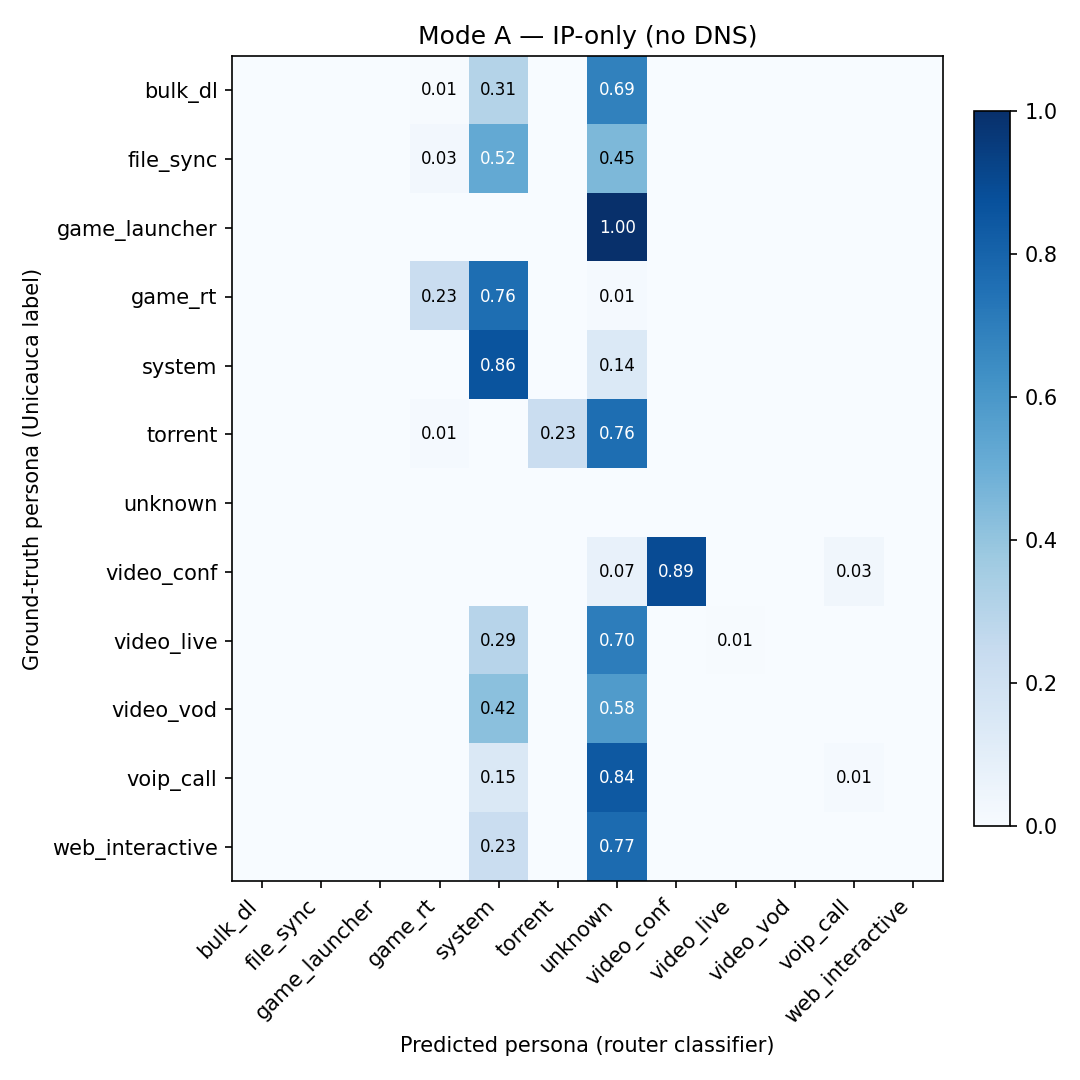
\includegraphics[width=0.48\textwidth]{../results/blind_test_ubuntu/report/confusion_modeA.png}\hfill
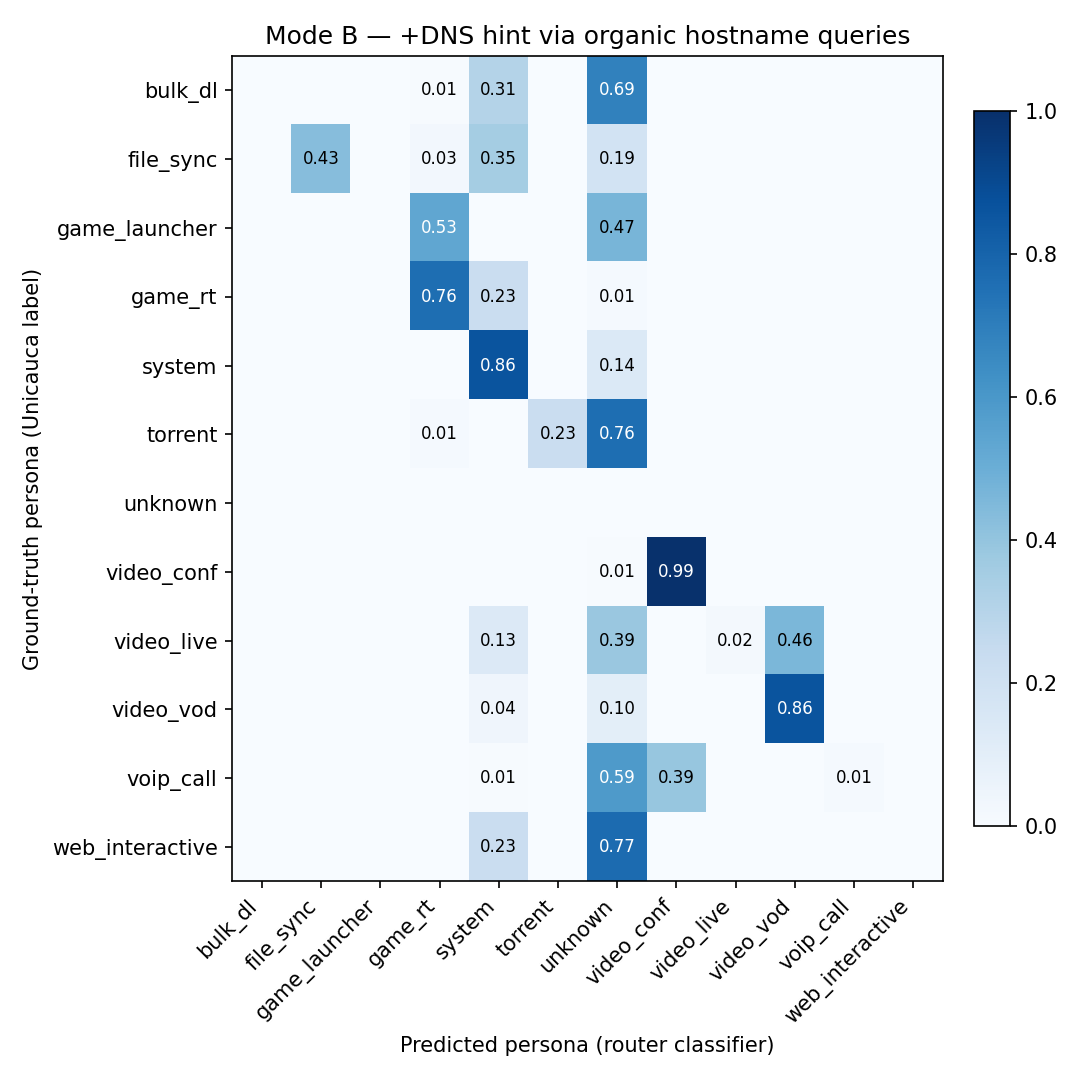
\includegraphics[width=0.48\textwidth]{../results/blind_test_ubuntu_v2/report/confusion_modeB.png}
\caption{Confusion matrices, Ubuntu testbed. Left: Mode~A (port +
behavior, no DNS). Right: Mode~B with the 585-catalog DNS sniffer.
Each cell is the row-normalised fraction of flows of the given
ground-truth class predicted as the column class.}
\end{figure}

\section{Hardware Resource Overhead}

\begin{table}[h]
\centering
\caption{Router resource consumption during the in-vivo Mode~B run.
Sampling: 1\,Hz over the entire $\sim$110-minute test; system samples
include the daemon plus Wi-Fi, NAT, and the kernel.}
\begin{tabular}{l|ccc}
\toprule
\textbf{Metric} & \textbf{p50} & \textbf{p95} & \textbf{max} \\
\midrule
System CPU \%       & 25.4 & 46.3 & 92.8 \\
mycoflowd CPU \%    & 9.5  & 14.7 & 26.1 \\
Memory used \%      & 57.0 & 58.9 & 60.5 \\
Conntrack entries   & 554  & 785  & 1{,}023 \\
\midrule
mycoflowd RSS (KB)  & \multicolumn{3}{c}{\textbf{384 (constant)}} \\
Daemon crashes      & \multicolumn{3}{c}{0 / 4{,}914} \\
Flash writes (mtd)  & \multicolumn{3}{c}{0} \\
\bottomrule
\end{tabular}
\end{table}

\begin{figure}[h]
\centering
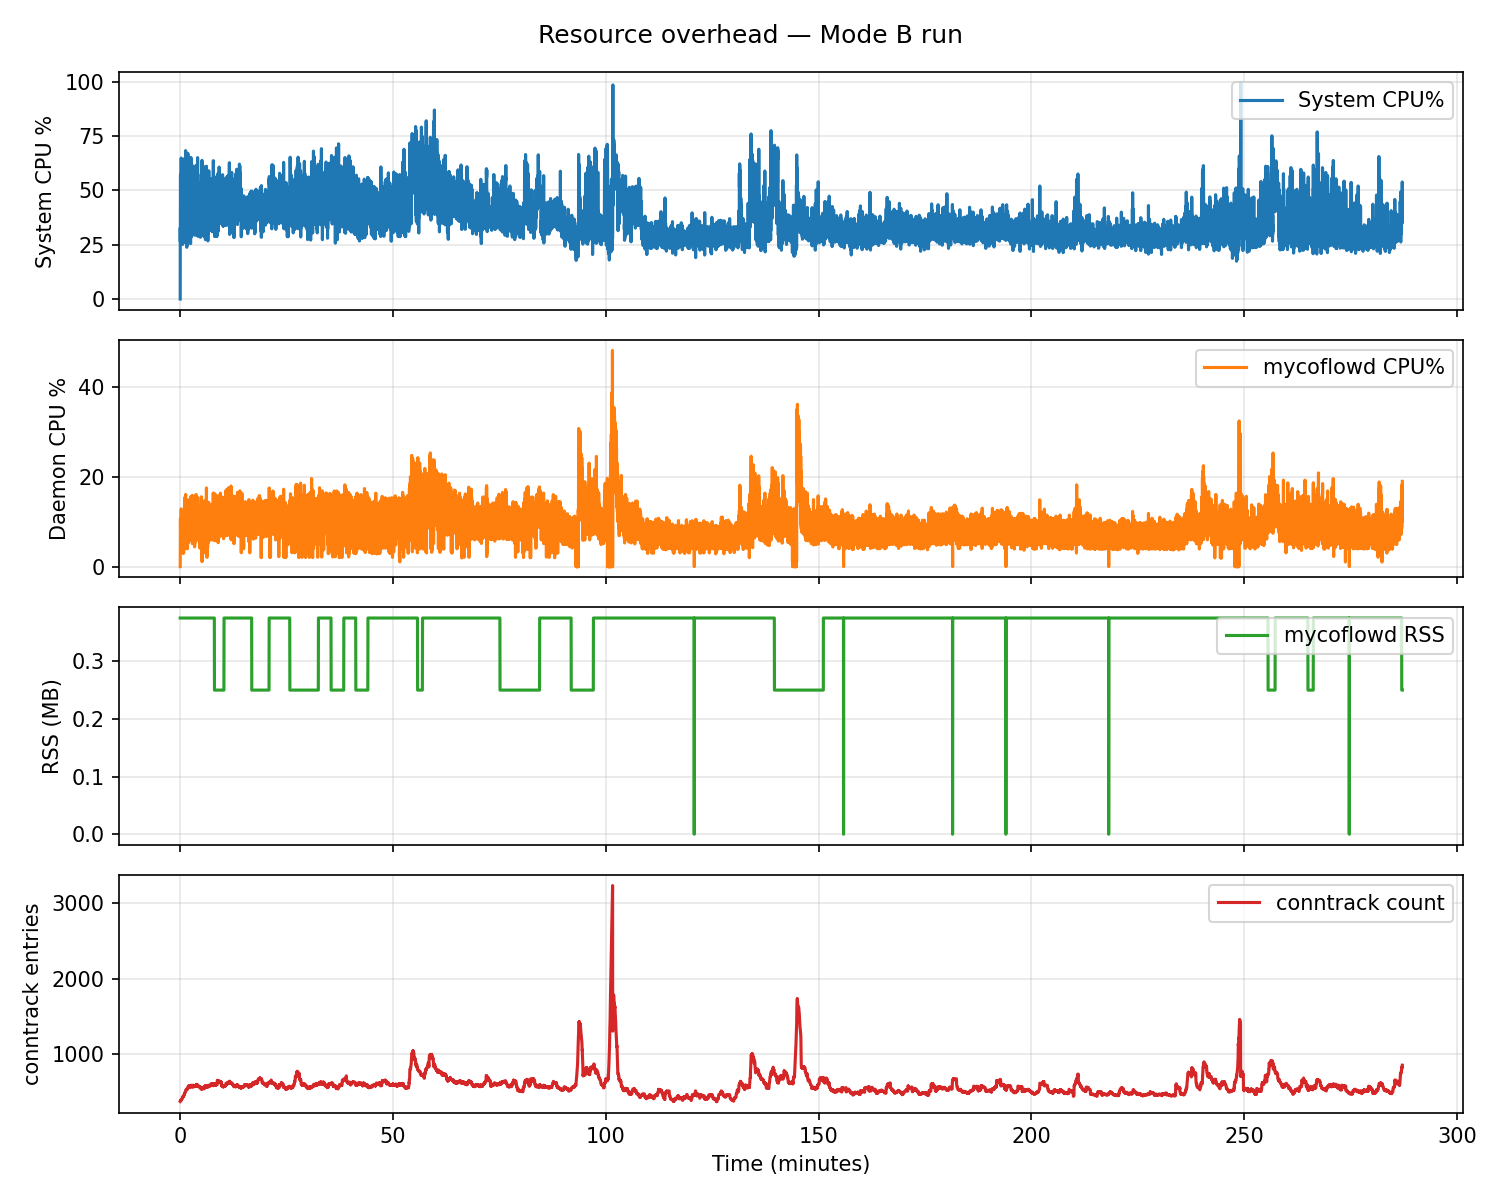
\includegraphics[width=0.7\textwidth]{../results/blind_test_ubuntu_v2/report/resources_modeB.png}
\caption{4-panel resource timeline: system CPU\%, daemon CPU\%, daemon
RSS (constant 384\,KB), conntrack entry count.}
\end{figure}

\section{Temporal Generalization}

\begin{table}[h]
\centering
\caption{Offline temporal split on the Unicauca dataset.}
\begin{tabular}{l|cc|c}
\toprule
\textbf{Predictor} & \textbf{Apr--May} & \textbf{June (held-out)} & $\boldsymbol{\Delta}$ \\
\midrule
Port + behavior      & 42.95\% & 42.51\% & $-$0.44\,pt \\
Port + behavior + DNS& 47.43\% & 47.04\% & $-$0.39\,pt \\
\bottomrule
\end{tabular}
\end{table}

Both gaps are within $\pm 0.5$\,pt of zero, well below the typical
$\pm 2$\,pt threshold used to flag temporal overfitting. The heuristic
decisions encoded in MycoFlow generalize across the calibration
boundary, supporting the claim that the system is production-ready
rather than tuned to a specific trace window.

\section{Reproducibility}

Every figure and number in this report is regenerable from the
repository:
\begin{itemize}
\item \texttt{scripts/dataset/prepare\_blind\_sample.py} writes the
121\,KB pre-sample (replaces the 1.2\,GB CSV reload at every run).
\item \texttt{scripts/dataset/router\_blind\_test.py} runs each mode.
\texttt{MYCOFLOW\_SSH\_KEYAUTH=1} for key auth (Ubuntu testbed),
\texttt{MYCOFLOW\_TCP\_OPEN=1} to drop the WSL-conservative TCP-port
whitelist.
\item \texttt{scripts/dataset/router\_blind\_analyze.py} writes the
Wilson CIs, McNemar tables, confusion-matrix PNGs, and resource
timeline PNGs from the JSONL outputs.
\item \texttt{scripts/dataset/temporal\_split\_validate.py} produces
the temporal-split table.
\end{itemize}

The repository tag at the time of submission contains:
\begin{itemize}
\item Daemon source (12 modules, $\sim$3\,K LoC C11, musl
static-pie aarch64 binary, 199\,KB).
\item Test scripts (Python 3, no third-party SSH binaries required on
the test host when SSH keys are provisioned).
\item All five runs' raw JSONL outputs (one row per flow tested),
the resource-monitor JSONL files, and the analyzer-generated PNG
figures.
\item This report and the IEEE TCE submission paper.
\end{itemize}

\end{document}
